\documentclass[border=6pt]{standalone}
\usepackage{tikz}
\usetikzlibrary{arrows.meta,positioning}
\begin{document}
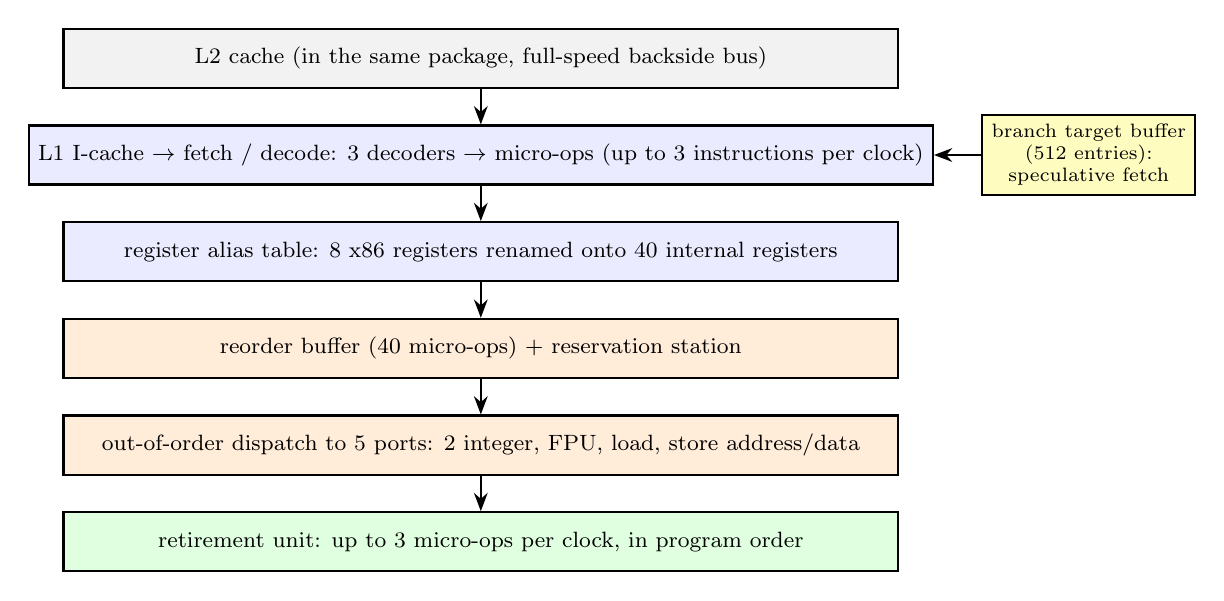
\begin{tikzpicture}[>=Stealth,font=\small,node distance=0.45cm,
 b/.style={draw,thick,minimum width=10.6cm,minimum height=0.75cm,align=center,font=\footnotesize}]
\node[b,fill=gray!10] (l2) {L2 cache (in the same package, full-speed backside bus)};
\node[b,fill=blue!8,below=of l2] (fd) {L1 I-cache $\to$ fetch / decode: 3 decoders $\to$ micro-ops (up to 3 instructions per clock)};
\node[b,fill=blue!8,below=of fd] (rat) {register alias table: 8 x86 registers renamed onto 40 internal registers};
\node[b,fill=orange!15,below=of rat] (rob) {reorder buffer (40 micro-ops) + reservation station};
\node[b,fill=orange!15,below=of rob] (ex) {out-of-order dispatch to 5 ports: 2 integer, FPU, load, store address/data};
\node[b,fill=green!12,below=of ex] (ret) {retirement unit: up to 3 micro-ops per clock, in program order};
\foreach \a/\c in {l2/fd,fd/rat,rat/rob,rob/ex,ex/ret} \draw[->,thick] (\a) -- (\c);
\node[draw,thick,fill=yellow!25,font=\scriptsize,align=center,right=0.6cm of fd] (btb) {branch target buffer\\(512 entries):\\speculative fetch};
\draw[->,thick] (btb) -- (fd);
\end{tikzpicture}
\end{document}
